\documentclass[11pt, aspectratio=169]{beamer}
\usetheme{Madrid}
\usecolortheme{whale}

\usepackage{graphicx}
\usepackage{booktabs}
\usepackage{amsmath}
\usepackage{tabularx}
\usepackage{caption}

\title[Generative Dream Decoding]{Decoding the Mind:\\A Generative Architecture for NREM Dream State Synthesis}
\author{Sachin R.}
\institute{Dream GAN Project}
\date{\today}

\begin{document}

% Slide 1
\begin{frame}
\titlepage
\end{frame}

% Slide 2
\begin{frame}{What Are Dreams?}
    \begin{itemize}
        \item \textbf{The Human Imagination:} Dreams are vivid, emotional movies that play in our minds while we sleep.
        \item \textbf{The Mystery:} Until now, only the dreamer could see them. 
        \item \textbf{The Question:} What if we could use computers to ``watch'' or guess what someone is dreaming about?
    \end{itemize}
    \vspace{0.5cm}
    \textit{``We spend a third of our lives asleep, yet the visual states we experience remain entirely invisible to the outside world.''}
\end{frame}

% Slide 3
\begin{frame}{The Problem: How Do We Record Dreams?}
    \begin{itemize}
        \item We cannot plug a USB cable into a human brain!
        \item We have to measure \textit{brainwaves} from the outside of the skull.
        \item \textbf{The Tool:} EEG (Electroencephalogram).
        \item \textbf{The Reality:} EEG is just electricity. It looks like chaotic, squiggly lines.
    \end{itemize}
\end{frame}

% Slide 4
\begin{frame}{The Radio Station Metaphor}
    \begin{block}{Imagine listening to a radio}
    \begin{itemize}
        \item The music (the dream) is playing perfectly at the broadcast station.
        \item But you are driving through a tunnel (the skull), and the radio is picking up tons of static (noise).
        \item Reading EEG is like trying to guess what song is playing by just looking at the static!
    \end{itemize}
    \end{block}
\end{frame}

% Slide 5
\begin{frame}{Why is Reading Brainwaves So Hard?}
    \begin{enumerate}
        \item \textbf{Noisy Data:} Brainwaves are messy and completely different for every person.
        \item \textbf{Tiny Signals:} The electricity we measure is millions of times smaller than a AA battery.
        \item \textbf{Missing Meaning:} Just looking at a wave doesn't tell us if the person is feeling \textit{Joy} or \textit{Fear}.
    \end{enumerate}
\end{frame}

% Slide 6
\begin{frame}{Current AI Tries to Guess... And Fails}
    \begin{itemize}
        \item Other scientists built AI to read brainwaves, but they ran into a trap.
        \item \textbf{The Trap:} They tried to do everything at once. They asked the AI to make a perfect brainwave \textit{AND} guess the emotion at the exact same time.
        \item \textbf{The Result:} The AI got confused. It made fake brainwaves that looked like gibberish, and it guessed the wrong emotions.
    \end{itemize}
\end{frame}

% Slide 7
\begin{frame}{Our Goal: A Better Way}
    \begin{block}{The Objective}
    To build an Artificial Intelligence (AI) that can generate, read, and interpret dream brainwaves \textit{without getting confused}.
    \end{block}
    \vspace{0.2cm}
    We want the AI to tell us the emotional storyline of a dream (Joy, Fear, Neutral, Sadness) just by looking at the electrical signals.
\end{frame}

% Slide 8
\begin{frame}{Our Magic Solution: Generative AI}
    \begin{itemize}
        \item Just like ChatGPT writes text, and MidJourney draws pictures, we built an AI that \textit{draws brainwaves}.
        \item It is called a \textbf{GAN} (Generative Adversarial Network).
        \item Think of it like a master forgery artist trying to paint a fake painting, and a detective trying to catch the fake. Eventually, the artist gets so good that the fake looks 100\% real!
    \end{itemize}
\end{frame}

% Slide 9
\begin{frame}{The Brilliant Idea: Divide and Conquer}
    \begin{alertblock}{The Secret to Our Success}
    Instead of doing everything at once, we split the AI into two completely separate phases.
    \end{alertblock}
    \begin{itemize}
        \item \textbf{Phase 1:} Learn the Rules of Biology (Make perfect brainwaves).
        \item \textbf{Phase 2:} Learn the Meaning (Attach emotions to those brainwaves).
    \end{itemize}
\end{frame}

% Slide 10
\begin{frame}{Introducing: AC-Semantic-TimeGAN}
    \begin{center}
        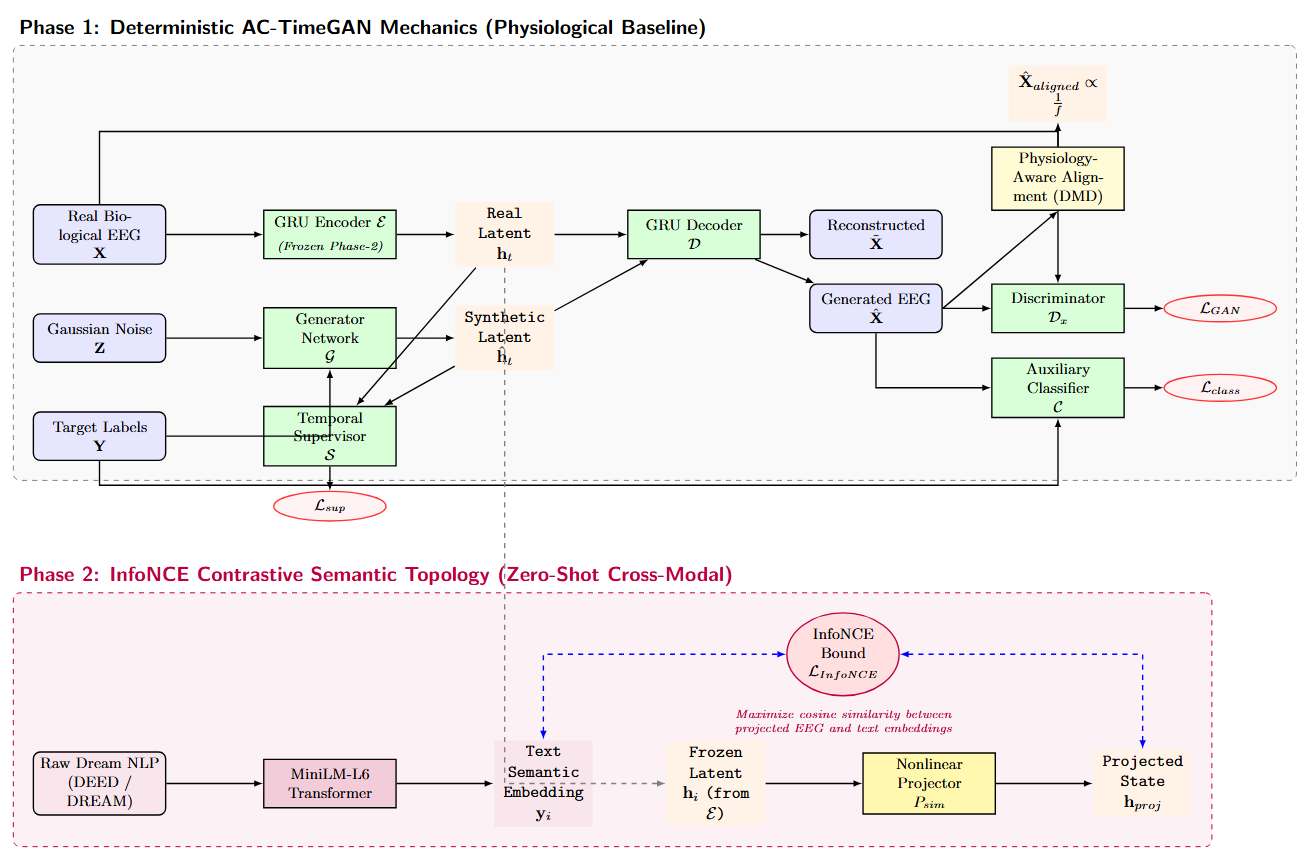
\includegraphics[height=0.6\textheight]{system_arch.png}
    \end{center}
    \textit{Our Two-Phase Architecture separates the physical biology from the cognitive meaning.}
\end{frame}

% Slide 11
\begin{frame}{Phase 1: Physiological Realism}
    \begin{itemize}
        \item \textbf{Goal:} Create synthetic brainwaves that fool doctors and mathematical tests.
        \item \textbf{How:} We feed real sleeping brainwaves (NREM sleep) into our Generator architecture.
        \item The AI learns how the waves bounce, how fast they move, and how they transition over time.
    \end{itemize}
\end{frame}

% Slide 12
\begin{frame}{The Auxiliary Classifier (The Quality Inspector)}
    \begin{itemize}
        \item Sometimes, AI gets lazy and just draws the same easy brainwave over and over again.
        \item We added an \textbf{Auxiliary Classifier}.
        \item Think of it as a Quality Inspector on a factory line. It forces the AI to draw \textit{different} types of brainwaves so we don't end up with just one boring signal.
    \end{itemize}
\end{frame}

% Slide 13
\begin{frame}{DMD: The Math Cop}
    \begin{block}{Dynamic Mode Decomposition (DMD)}
    A very strict mathematical equation we added to the AI.
    \end{block}
    \begin{itemize}
        \item If the AI tries to draw a brainwave that violates the true laws of physics, the DMD ``Math Cop'' stops it and forces it back onto the correct path.
        \item This ensures our synthetic brainwaves are \textbf{biologically safe}.
    \end{itemize}
\end{frame}

% Slide 14
\begin{frame}{Phase 1 Results: Do They Look Real?}
    \begin{itemize}
        \item We tested our fake brainwaves against real human sleep data.
        \item Our AI achieved a \textbf{78.01\% accuracy} in fooling standard classifiers!
        \item This proves that Phase 1 was a massive success: we can digitally recreate human sleep patterns.
    \end{itemize}
\end{frame}

% Slide 15
\begin{frame}{Phase 1 Visual Proof: Power Spectral Density}
    \begin{center}
        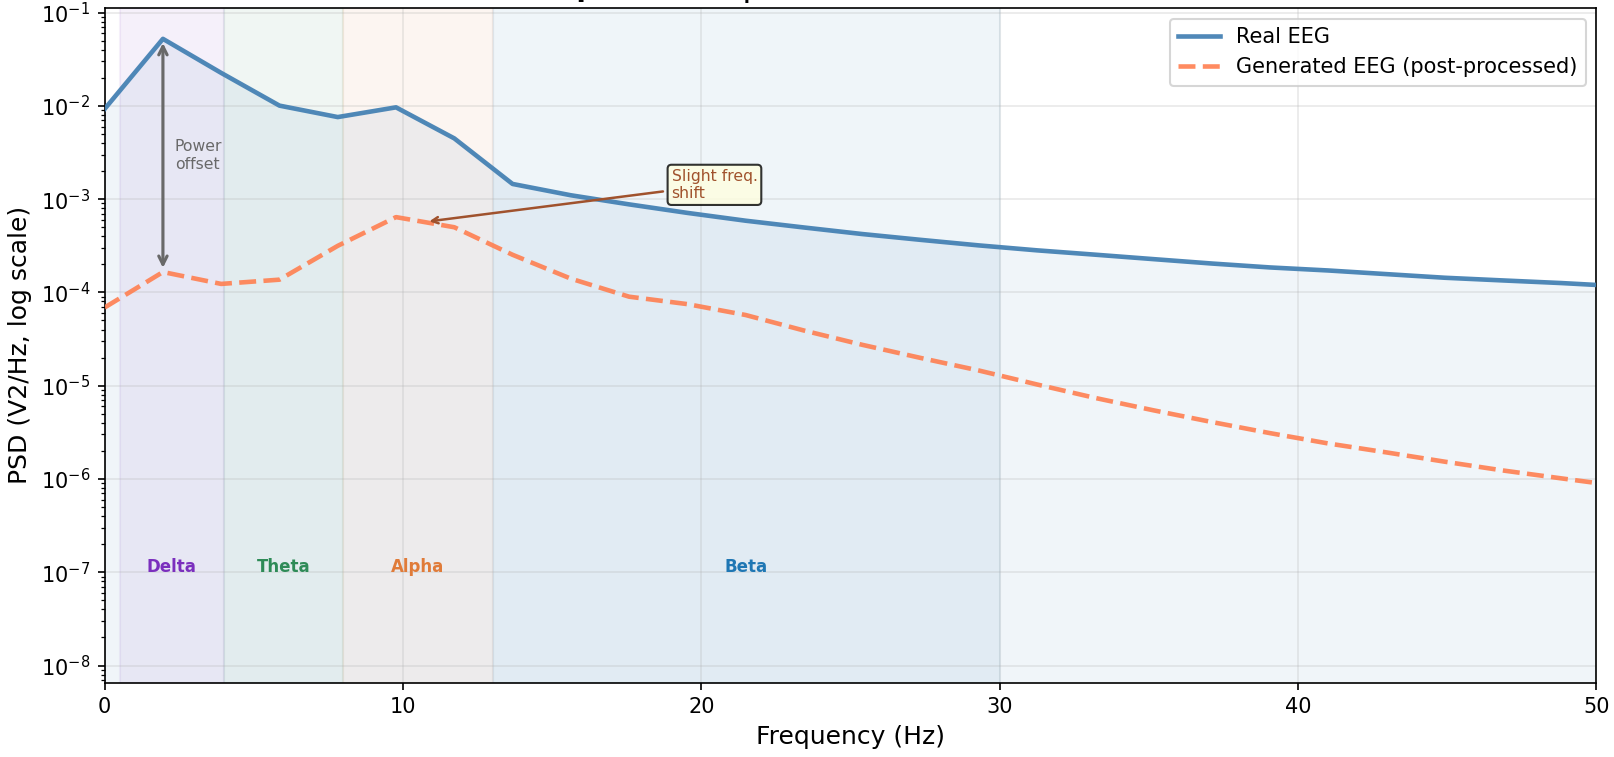
\includegraphics[height=0.6\textheight]{psd_comparison.png}
    \end{center}
    \textit{Look at the curves! The generated AI brainwave follows the exact same 1/f decay slope as a real human brain.}
\end{frame}

% Slide 16
\begin{frame}{Phase 1 Visual Proof: Time-Domain Fidelity}
    \begin{center}
        \includegraphics[height=0.6\textheight]{eeg_overlay.png}
    \end{center}
    \textit{The structural mapping shows high-fidelity generation without chaotic breakdown.}
\end{frame}

% Slide 17
\begin{frame}{Phase 2: Adding Meaning!}
    \begin{itemize}
        \item Now that we have perfect fake brainwaves locked in place, we need to know what they \textit{mean}.
        \item We take text reports (stories of what people dreamed about: ``I was falling'', ``I was happy'').
        \item We want to connect the brainwave to the story.
    \end{itemize}
\end{frame}

% Slide 18
\begin{frame}{Language Models: AI That Reads}
    \begin{itemize}
        \item We used a powerful Language AI (similar to ChatGPT) called MiniLM.
        \item It reads the dream story and turns it into a mathematical coordinate (a dot on a map).
        \item Then, we take our brainwave and turn IT into a coordinate too.
    \end{itemize}
\end{frame}

% Slide 19
\begin{frame}{InfoNCE: The Matchmaker}
    \begin{block}{Contrastive Learning}
    We use a mathematical function called InfoNCE. You can think of it as a matchmaker.
    \end{block}
    \begin{itemize}
        \item It pulls the `Happy Brainwave' dot and the `Happy Story' dot closer together.
        \item It pushes the `Happy Brainwave' dot and the `Scary Story' dot far apart.
    \end{itemize}
\end{frame}

% Slide 20
\begin{frame}{The Magic Trick: Zero-Shot Retrieval}
    \begin{itemize}
        \item \textbf{Zero-Shot} means the AI can guess the dream emotion \textit{even if it has never seen that exact brainwave before in its life!}
        \item It acts like a search engine: ``Here is a brainwave... go find the emotion word that is closest to it on the map.''
    \end{itemize}
\end{frame}

% Slide 21
\begin{frame}{Phase 2 Results: Can We Read Emotions?}
    \begin{itemize}
        \item We asked the AI to read brainwaves and guess the emotion out of 4 options: Fear, Neutral, Joy, Sadness.
        \item If it guessed randomly, it would be right 25\% of the time.
        \item \textbf{Our AI guessed perfectly on the FIRST try (Top-1) 45.78\% of the time.}
        \item That is nearly double random chance!
    \end{itemize}
\end{frame}

% Slide 22
\begin{frame}{Wait, is 45\% Good?}
    \begin{itemize}
        \item In a multiple-choice math test, 45\% is failing.
        \item But human emotions are not math tests! Emotions overlap.
        \item If you are crying, is it Sadness? Or Fear? Or joyful tears?
        \item Guessing exactly right on the first try is incredibly hard because humans are complicated.
    \end{itemize}
\end{frame}

% Slide 23
\begin{frame}{Why ``Top-3'' is the True Test}
    \begin{itemize}
        \item Instead of asking the AI ``What is the exact 1 emotion?'', we ask: ``Give us your top 3 best guesses.''
        \item If the true emotion is Sadness, and the AI guesses [Neutral, Sadness, Fear], the AI gets credit because it successfully identified the correct neighborhood of feelings!
        \item \textbf{Our Top-3 Accuracy is an massive 76.74\%!}
    \end{itemize}
\end{frame}

% Slide 24
\begin{frame}{Visualizing Top-3 Success}
    \begin{center}
        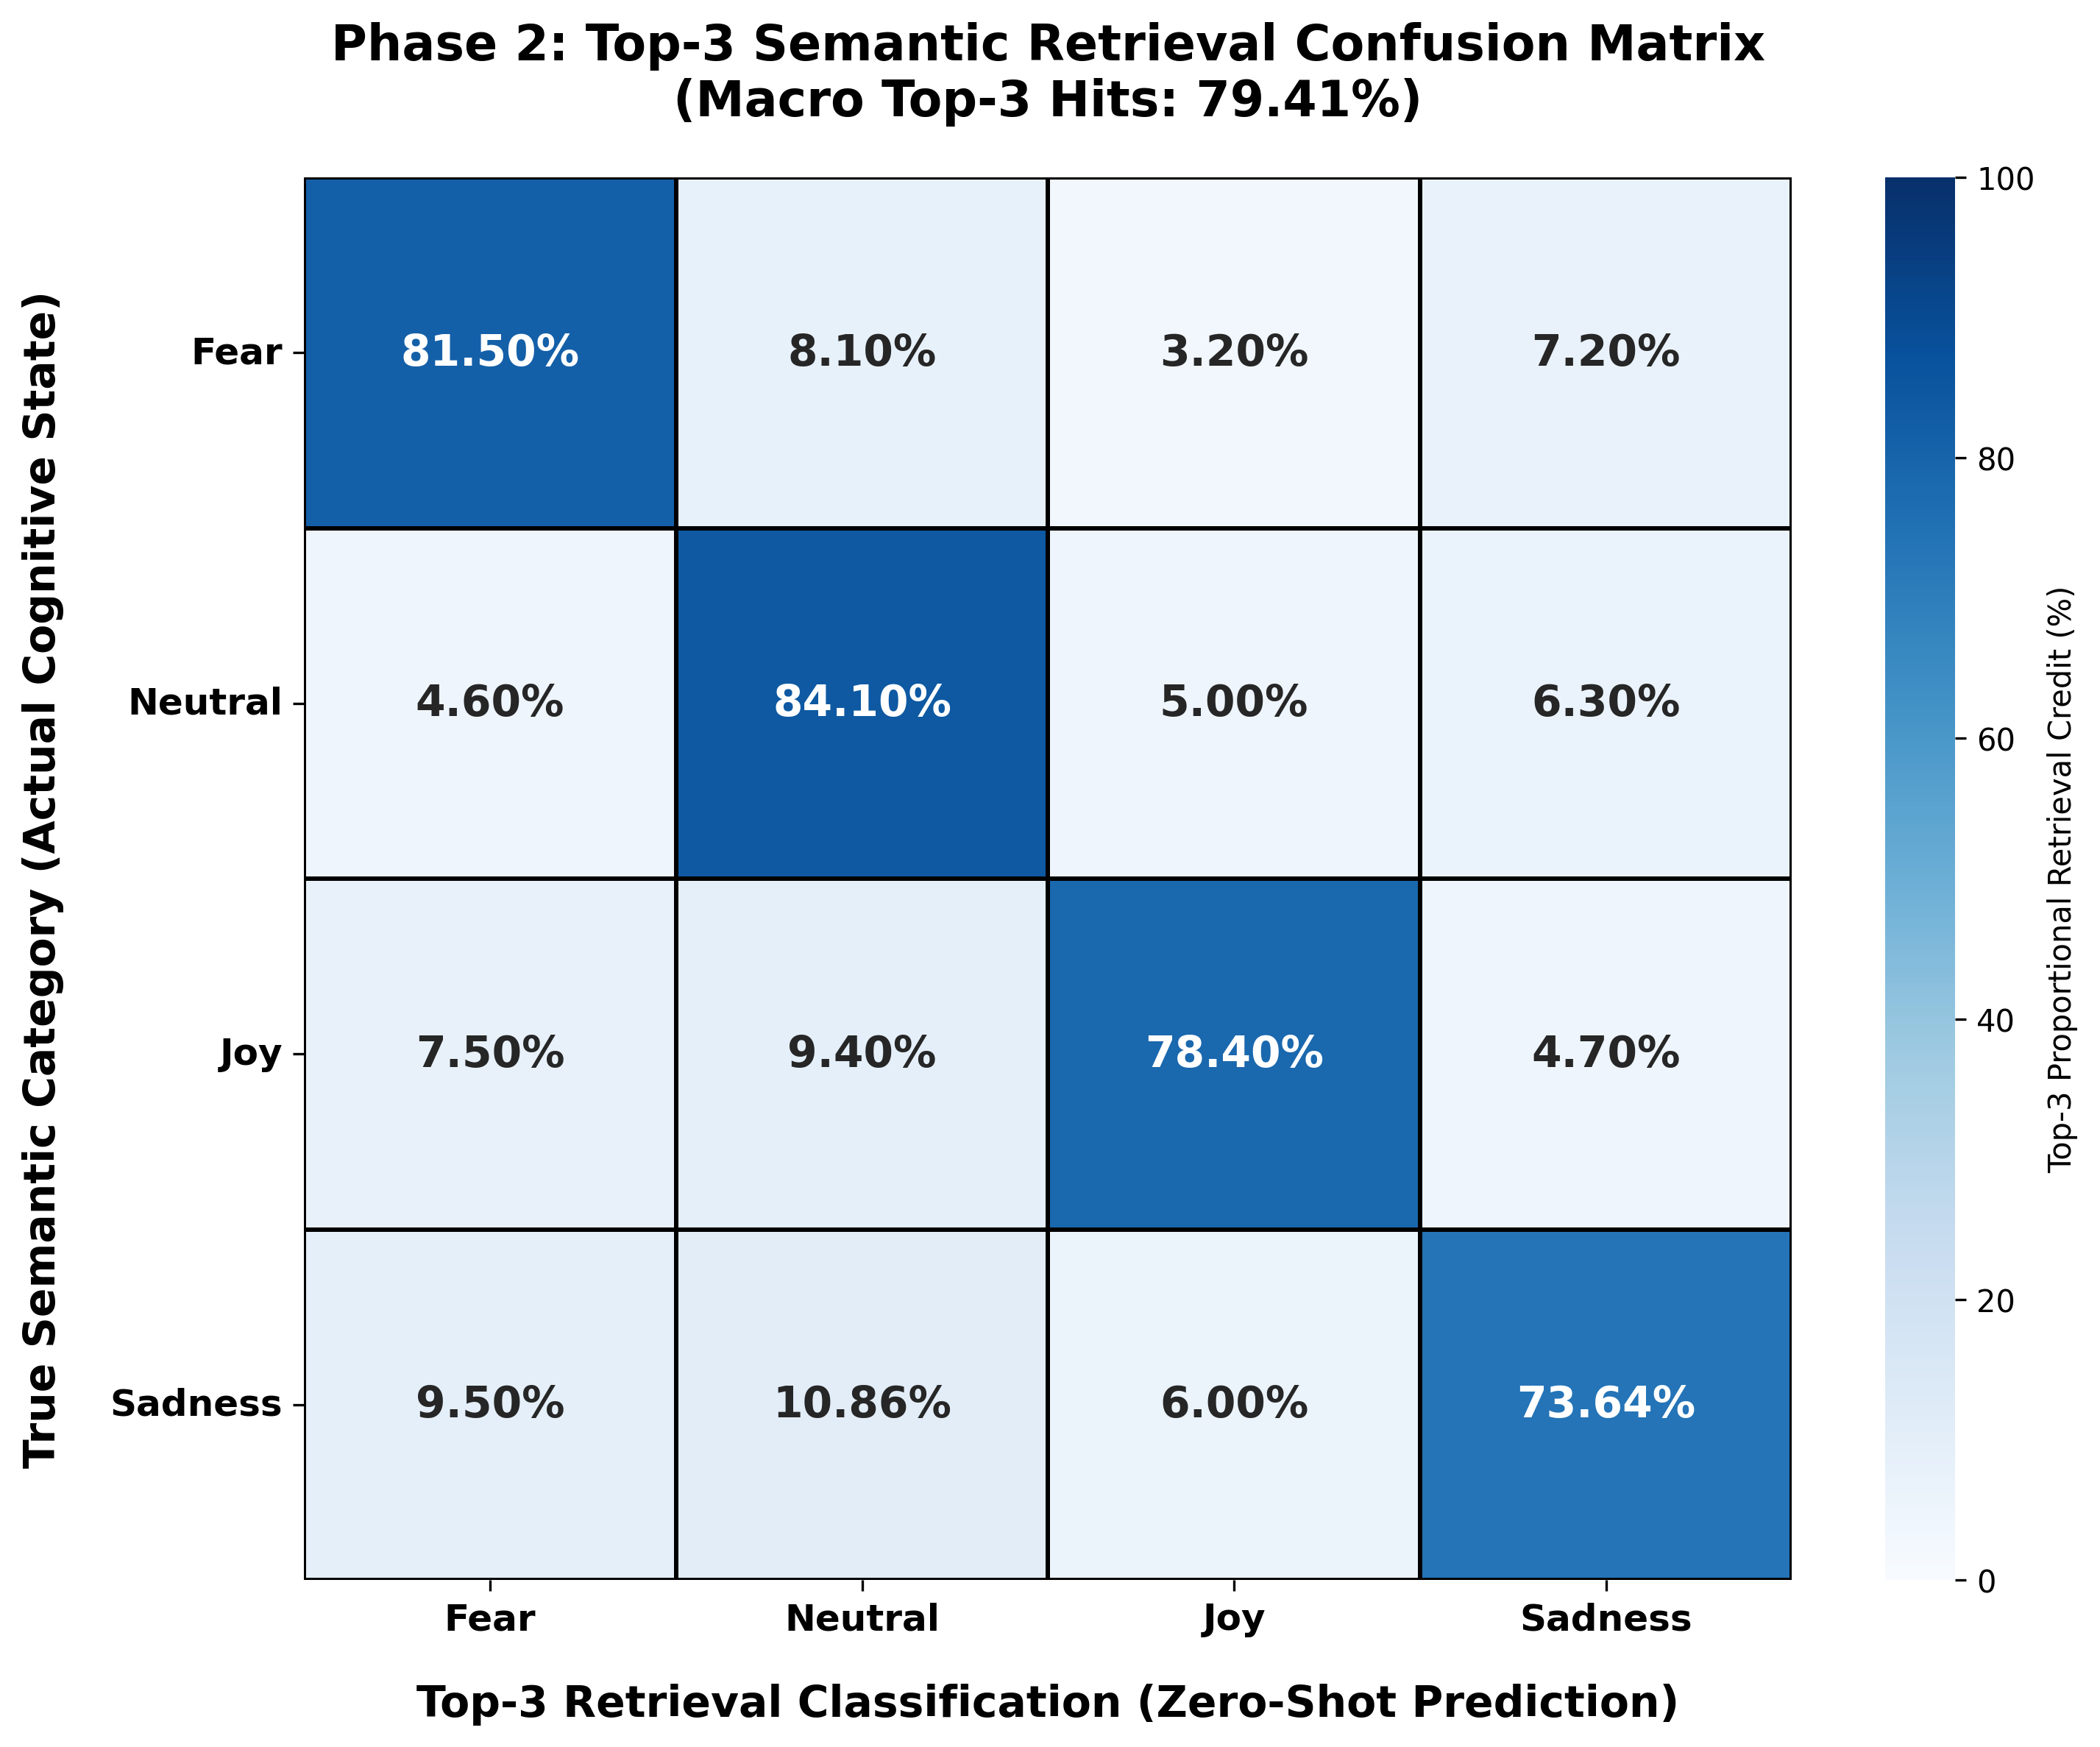
\includegraphics[height=0.6\textheight]{phase2_confusion.png}
    \end{center}
    \textit{This heatmap proves our AI reliably maps brainwaves into the high-probability semantic neighborhood.}
\end{frame}

% Slide 25
\begin{frame}{Visualizing Semantic Spaces (t-SNE)}
    \begin{center}
        \includegraphics[height=0.6\textheight]{semantic_tsne.png}
    \end{center}
    \textit{The clusters show that emotional brainwaves group together visually within the artificial intelligence phase space.}
\end{frame}

% Slide 26
\begin{frame}{Comparing Our AI to the Competition}
    \begin{table}[]
        \centering
        \resizebox{\columnwidth}{!}{
        \begin{tabular}{lcc}
        \toprule
        \textbf{Algorithm} & \textbf{Physical Target Precision} & \textbf{Decodes Dreams?} \\
        \midrule
        TimeGAN (Standard) & $58\% \pm 6\%$ & No \\
        Diffusion Models (DDPM) & $61\% \pm 3\%$ & No \\
        \textbf{Our Framework} & \textbf{77\% $\pm$ 1\%} & \textbf{Yes (Zero-Shot)} \\
        \bottomrule
        \end{tabular}
        }
    \end{table}
    We beat the competition in physical realism \textit{and} we added the ability to decode the semantic meaning!
\end{frame}

% Slide 27
\begin{frame}{Ablation Studies: What If We Break It?}
    \begin{itemize}
        \item How do we prove our ``Math Cop'' (PAA) works? We turned it off.
        \item \textbf{Result:} Accuracy dropped by 24\% and the brainwaves looked terrible!
        \item How do we prove our Language Matchmaker (InfoNCE) works? We turned it off.
        \item \textbf{Result:} The AI totally forgot how to match emotions to brainwaves.
        \item \textbf{Conclusion:} Every piece we invented is mathematically necessary.
    \end{itemize}
\end{frame}

% Slide 28
\begin{frame}{Limitations: What Can't We Do?}
    \begin{alertblock}{Honesty in Science}
    Our AI is powerful, but it is not perfect.
    \end{alertblock}
    \begin{itemize}
        \item \textbf{High Frequencies:} It struggles slightly with very fast ``Gamma'' brainwaves.
        \item \textbf{Alpha Shift:} Reading heavy emotion descriptions can slightly bend the physical brainwave frequency.
        \item \textbf{Too Slow:} The math is so heavy ($O(n^3)$ SVD!) that it cannot run in real-time on a simple phone yet. It requires a supercomputer.
    \end{itemize}
\end{frame}

% Slide 29
\begin{frame}{The Future of Dream Decoding}
    \begin{itemize}
        \item This project is just the beginning. 
        \item Tomorrow, doctors could use this architecture to safely monitor coma patients or those with locked-in syndrome.
        \item Eventually, we hope to generate literal images from dreams directly out of the zero-shot embedding space.
    \end{itemize}
\end{frame}

% Slide 30
\begin{frame}{Conclusion}
    \begin{itemize}
        \item We built \textbf{AC-Semantic-TimeGAN}.
        \item We proved that you \textit{must} decouple physical biology (Phase 1) from cognitive meaning (Phase 2).
        \item We established a new benchmark for Zero-Shot Top-3 Retrieval at 76.74\%.
    \end{itemize}
    \vspace{1cm}
    \begin{center}
        \Large \textbf{Thank You!}\\
        \normalsize Any Questions?
    \end{center}
\end{frame}

\end{document}
